\section{Introduction}
\label{sec:introduction}

% state the learning objective 
\paragraph{} The objective of this laboratory assignment is to study the circuit detailed in figure 1, looking at it's operation in function of the sinusoidal voltage source $v_S$.

In Section 2 we wil perform the Simulation Analysis of the circuit, making use of the NGSpice software. We will simulate the circuit to obtain, among other things, the natural and the forced responses of the circuit.

In Section 3 we will perform the Theoretical Analysis, analogous to the previous section, we will do the analysis of the circuit making use of theoretical methods, such as the Thevenin and the Phasor Analysis.

In Section 4 we shall compare the results obtained in Sections 2 and 3, and comment on the differences (should they exist) and draw our conclusions. 

\begin{figure}[h] \centering
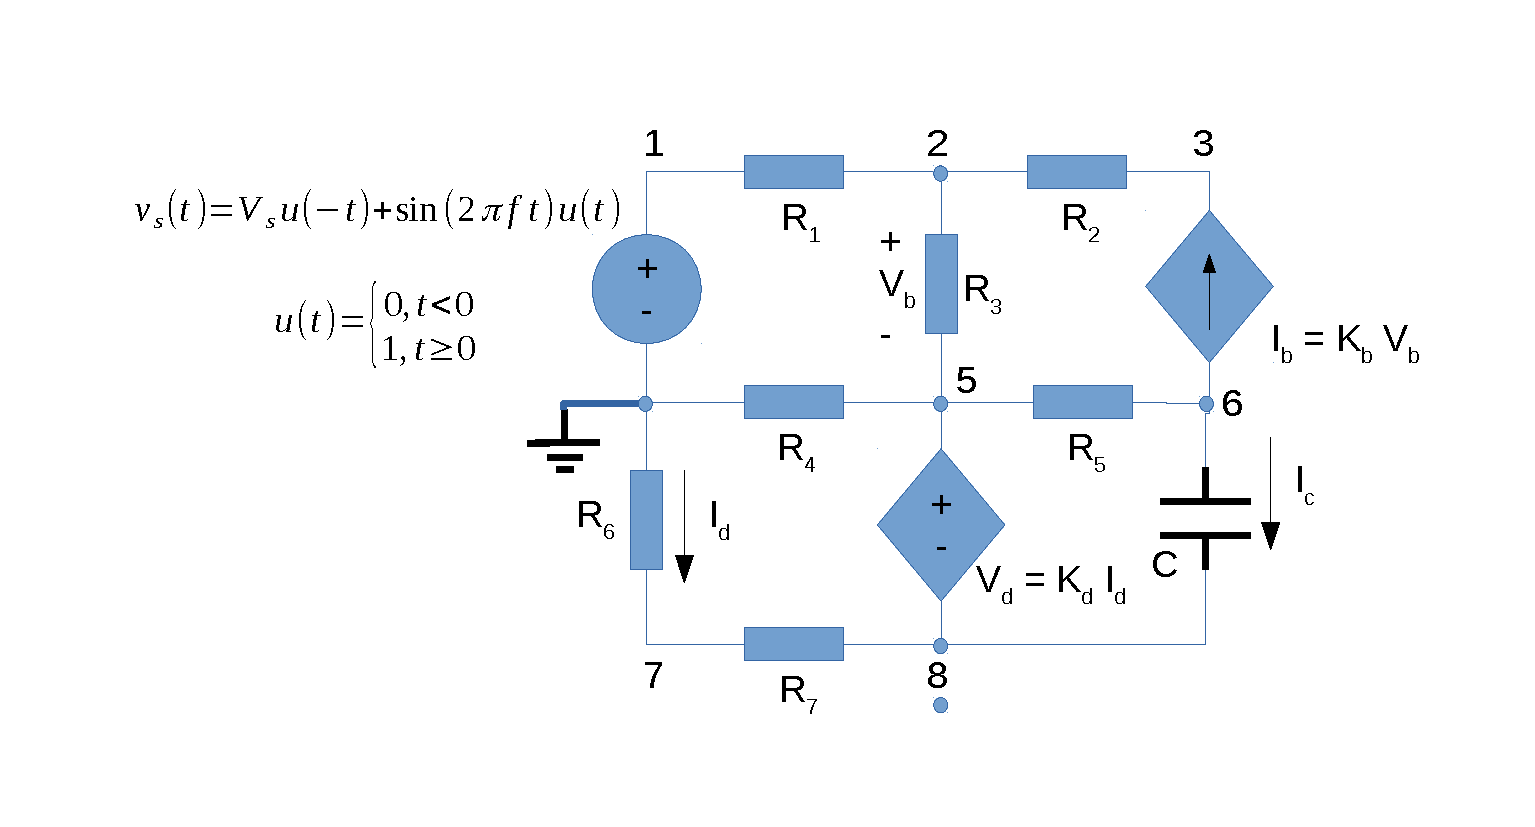
\includegraphics[width=0.5\linewidth]{circuit.pdf}
\caption{Circuit to be analyzed in the laboratory assignment.}
\label{fig:rc}
\end{figure}

